\section{Основы линейной и нелинейной оптики.}

\subsection{Материальное уравнение линейной среды.}
\hspace*{2mm}
В основе взаимодействия света со средой лежит элементарный процесс возбуждения атома или молекулы вещества световым полем и последующего переизлучения света возбужденной частицей. Характер этого взаимодействия зависит от соотношения между величиной напряженности поля световой волны Е и характерной напряженностью внутриатомного поля  $E_{atom}$, определяющего силы связи оптических электронов (т.е. внешних, наиболее слабо связанных электронов) с ядром атома вещества. Оценка поля Е световой волны в случае не лазерных источников свет дает величину  $E<<E_{atom} $. При этом условии отклик атомного осциллятора на внешнее воздействие будет иметь линейный характер, а зависимость поляризованности Р = Р(Е) в случае изотропной среды может быть представлена в виде:
\begin{equation}\label{1:liner}
P(E) = \chi^{(1)}E
\end{equation}
где $ \chi^{(1)}$ – линейная восприимчивость среды, являющаяся безразмерной величиной и зависящая только от свойств среды \cite{achmanov2}. Материальное уравнение (\ref{1:liner}) является одним из соотношений, на которых базируется линейная оптика.  Но оно справедливо только при условии $E << E_{atom} $, а во слех остальных случаях является лишь некоторым приближением. 
\\
В мощных лазерных пучках можно получить напряженности уже сравнимые с $E_{atom} $. В случае когда поле Е, оставаясь меньше $E_{atom} $, приближается к нему по величине, поляризация среды перестает быть линейной функцией поля Е, и в этом случае материальное уравнение (\ref{1:liner}) должно быть заменено на другое.

\subsection{Материальное уравнение нелинейной среды.} 
\hspace*{2mm}
Теория нелинейно-оптических явлений строится на основе материальных уравнений и уравнений Максвелла  \cite{achmanov2}. Уравнения Максвелла для диэлектрической нейтральной немагнитной среды имеют вид
\begin{equation}\label{1:maxvel}
rot\vec{E} = - \frac{ 1 }{ c}\frac{\partial \vec{H} }{\partial t}
\hspace{20mm}
rot\vec{H} =  \frac{ 1 }{ c}\frac{\partial \vec{D} }{\partial t}
\hspace{20mm}
div\vec{H} = 0
\end{equation}где $ \vec{D} = \vec{E} + 4\pi \vec{P}$. Из уравнений Максвелла вытекает волновое уравнение
\begin{equation}\label{1:rot_maxvel}
rot(rot\vec{E}) + \frac{ 1 }{ c^2 }\frac{\partial^2 \vec{E} }{\partial t^2} = - \frac{ 4\pi }{ c^2 }\frac{\partial^2 \vec{P} }{\partial t^2}
\end{equation}которе в случае изотропной среды принимает вид
\begin{equation}\label{1:wave_eq}
\Delta\vec{E} - \frac{ 1 }{ c^2 }\frac{\partial^2 \vec{E} }{\partial t^2} =  \frac{ 4\pi }{ c^2 }\frac{\partial^2 \vec{P} }{\partial t^2}
\end{equation}
где $\vec{E}$ - напряженность электрического поля, а $\vec{P}$ - поляризация среды. Поляризация среды возникает под действием падающий световой волны и описывается материальным уравнением $\vec{P} = \vec{P}(\vec{E})$.
В анизотропном случае $\vec{P}(\vec{E})$ являеться тензорный величиной и может быть представлена в виде:
\begin{equation}\label{1:p_1}
P(E) = \chi^{(1)}E + \chi^{(2)}E^2 +\chi^{(3)}E^3\dots
\end{equation}
Коэффициенты $\chi^{(m)}, m \ge 2$ при членах разложения называются нелинейными восприимчивостями m-го порядка и являются уже размерными величинами. Таким образом, отклик среды на действие внешнего светового поля перестает быть линейным.  С математической точки зрения именно нелинейность материального уравнения является причиной нарушения принципа суперпозиции для световых волн в нелинейной среде. Из уравнений (\ref{1:rot_maxvel}), (\ref{1:wave_eq}) и (\ref{1:p_1}) непосредственно вытекает возможность генерации оптических гармоник и других нелинейно-оптических эффектов. Материальное уравнение вида  (\ref{1:wave_eq}), описывает изотропную нелинейную среду с безынерционным локальным откликом на световое поле. Аналогичное уравнение для анизотропной нелинейной диспергирующей среды является уже не только тензорным, но и имеет комплексную часть. Коэффициент восприимчивости $\chi^{(m)}$ представим в виде:
\begin{equation}\label{1:p_2}
\chi^{(m)} = Re(\chi^{(m)}) + iIm(\chi^{(m)})
\end{equation}и уже зависят от времени о координаты. Среды, обладающие таким свойством, называют средами с пространственной дисперсией. К их числу относятся некоторые типы кристаллов, а также плазма \cite{achmanov2}.

\subsection{Основные процессы и эффекты нелинейной оптики}
Физические причины, приводящие к появлению нелинейных оптических эффектов, достаточно многообразны. К ним можно отнести:
\begin{enumerate}
\item  Нелинейную рефракцию в оптически прозрачной среде, т.е. зависимость показателя преломления среды от амплитуды светового вектора;
\item  Нелинейный характер рассеяния света в среде при больших интенсивностях светового поля;
\item  Многофотонное поглощение интенсивного (атом вещества переходит из основного состояния в возбужденное при одновременном поглощении двух и более фотонов)
\item  Генерацию высших гармоник при переизлучении световой волны;
\item  Тепловые самовоздействия и др.
\end{enumerate}
\begin{figure}[h]
	\centering
	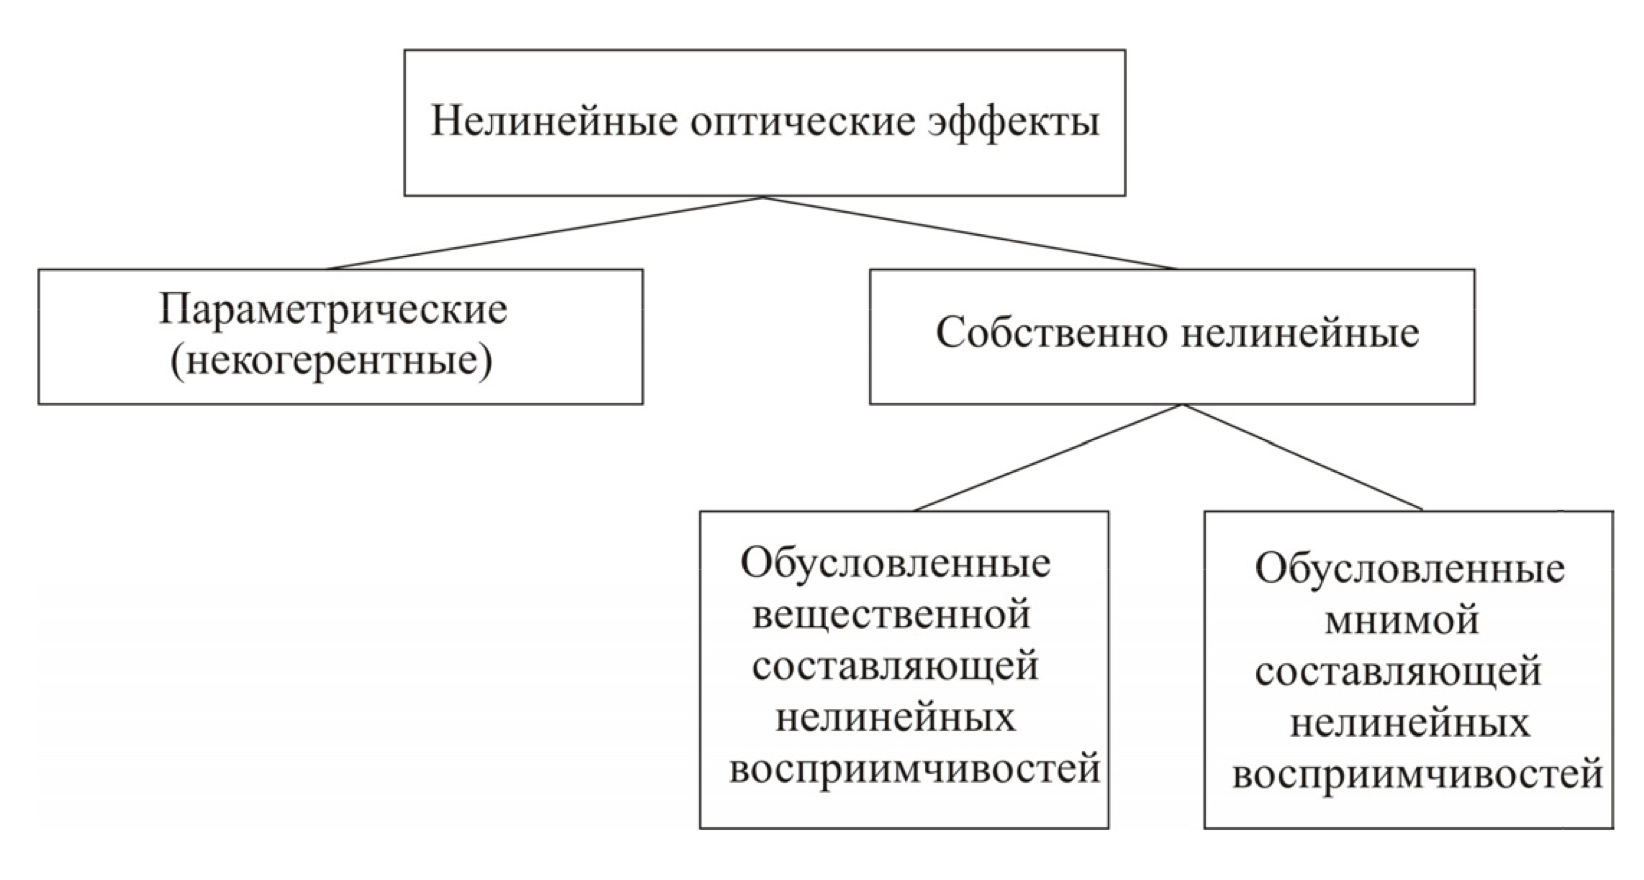
\includegraphics[width=0.7\linewidth]{images/classific.png}
	\caption{Классификация нелинейных оптических эффектов}
	\label{classific}
\end{figure}
К \textit{параметрическим явлениям} относятся:
\begin{enumerate}
\item   Электрооптический эффект, или эффект Поккельса (сообщение оптической анизотропии кристаллическим изотропным диэлектрикам без центра инверсии, помещенным в сильное однородное электрическое поле, при этом показатель преломления становится нелинейной функцией напряженности поля); является нелинейным эффектом второго порядка;
\item Эффект Керра (аналогичен эффекту Поккельса, но является нелинейным эффектом третьего порядка) и ряд других.
\end{enumerate}
К эффектам, \textit{обусловленным вещественной составляющей нелинейных восприимчивостей}, относятся:
\begin{enumerate}
\item  Эффекты генерации высших оптических гармоник, в частности, связанные с удвоением и утроением частоты света;
\item  Самовоздействие интенсивного светового пучка в нелинейных материалах (например, явление самофокусировки, при котором возникает перепад свойств среды в пучке и вне пучка, а его распространение приобретает волноводный, нитевидный характер, устраняющий геометрическую и дифракционную расходимость; при самофокусировке нарушается закон прямолинейного распространения света);
\item Оптический пробой среды, в основе которого лежит процесс качественного превращения прозрачной в сильно поглощающую среду с изменением агрегатного состояния при некотором значении интенсивности света;
\end{enumerate}
К эффектам, \textit{обусловленным мнимой составляющей нелинейных восприимчивостей}, относятся:
\begin{enumerate}
\item  Многофотонные процессы (фотоионизация и фотовозбуждение, гиперрассеяние света и другие), когда в элементарном акте взаимодействия света с атомом вещества участвует не один, а несколько фотонов; если мнимая составляющая линейной восприимчивости ответственна за однофотонные процессы, то мнимые составляющие восприимчивостей высших порядков – за многофотонные процессы;
\item  Вынужденное комбинационное рассеяние света, заключающееся в том, что интенсивное падающее излучение вызывает появление в оптической среде волны рассеянного стимулированного излучения на смещенных (комбинационных) частотах, характеристики которого имеют нелинейную зависимость от характеристик вынуждающего излучения;
\item Вынужденное рассеяние Мандельштама – Бриллюэна, при котором мощное световое излучение возбуждает в среде когерентные колебания молекул по закону бегущей волны, при этом происходит рассеяние света на образовавшейся периодической структуре (сверхзвуковой волне).
\end{enumerate}


\subsection*{Генерация второй оптической гармоники} 
\hspace{2mm}
Обсудим подробнее эффект удвоения частоты света в кристалле — генерации второй оптической гармоники \cite{achmanov2}. Данный эффект состоит в том, что под действием мощного лазерного излучения в нелинейном кристалле возникает излучение на удвоенной частоте.
\\
\hspace{2mm}
Пусть на квадратично-нелинейную среду воздействует монохроматическое поле с частотой $\omega$:
\begin{equation}\label{shg:e(t)}
A(t) = A\cos(\omega t)
\end{equation}Тогда нелинейная поляризация второго порядка будет пропорциональна полю во второй степени:
\begin{equation}\label{shg}
P(t)^{(2)} = \chi^{(1)}E(t)^2 = \frac{1}{2}\chi^{(1)}A^2 + \frac{1}{2}\chi^{(1)}A^2\cos(2\omega t)
\end{equation}Это значит, что поляризация будет иметь постоянную составляющую $ \frac{1}{2}\chi^{(1)}A^2$ , и переменную $\frac{1}{2}\chi^{(1)}A^2\cos(2\omega t)$, на удвоенной частоте $2\omega$. Первое слагаемое в (\ref{shg}) соответствует нелинейному процессу, который называется \textbf{оптическим выпрямлением}, а второе – \textbf{генерации второй гармоники}. 
\\
Происходит возбуждение волны поляризации на удвоенных частотах $2\omega_{1,2}$ (\textbf{генерация второй гармоники}, ГВГ), разностной $\omega_1 + \omega_2$(\textbf{генерация разностной частоты}, ГРЧ), суммарной $\omega_1 - \omega_2$ (\textbf{генерация суммарной частоты}, ГСЧ), и нулевой (\textbf{оптическое выпрямление}) частотах (рис. \ref{sghPictr}).
\begin{figure}[h]
	\centering
	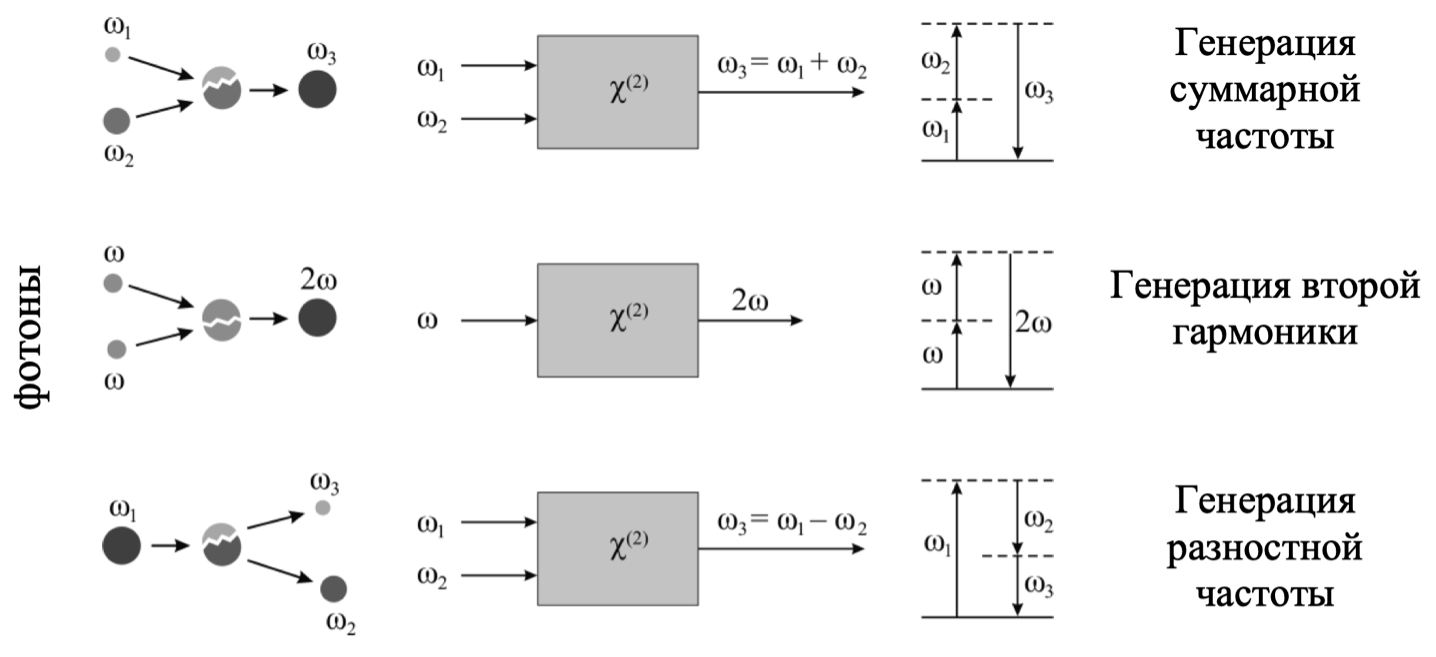
\includegraphics[width=0.7\linewidth]{images/shg.png}
	\caption{Схематическое представление нелинейно-оптических процессов второго порядка.}
	\label{sghPictr}
\end{figure}

\subsection*{Генерация третей оптической гармоники} 
Пусть на квадратично-нелинейную среду воздействует монохроматическое поле (\ref{shg:e(t)}) с частотой $\omega$. Тогда поляризация третьего порядка зависит от времени следующим образом:
\begin{equation}\label{thg}
P(t)^{(3)} = \chi^{(3)}E(t)^3 = \frac{1}{4}\chi^{(3)}A^3\cos(3\omega t) + \frac{3}{4}\chi^{(3)}A^3\cos(\omega t)
\end{equation}
То есть, происходит генерация третьей гармоники (THG) и переизлучение на исходной частоте (\textbf{самовоздействие света}) – см. рис. \ref{thg1}a, b. Поскольку, как правило, $\chi^{(3)}E^3 << \chi^{(2)}E^2$ то эффект THG в кубически-нелинейной среде очень мал, и на практике третью гармонику лазерного излучения получают путѐм последовательного удвоения частоты $\omega +  \omega \rightarrow 2\omega$, а затем сложения волн первой и второй гармоники: $\omega +  2\omega \rightarrow 3\omega$ в квадратично-нелинейной среде
\begin{figure}[h]
	\centering
	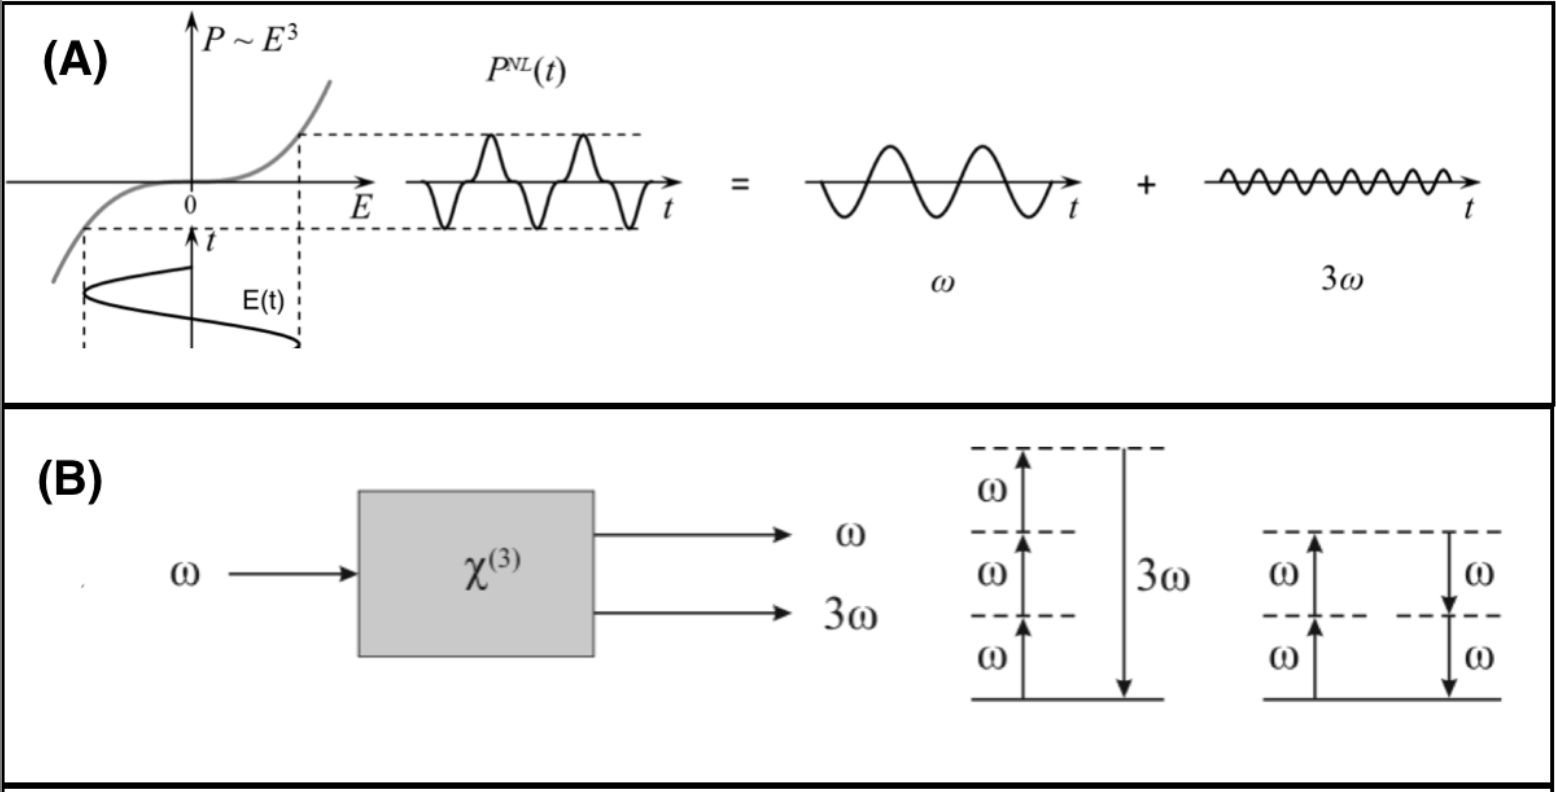
\includegraphics[width=0.8\linewidth]{images/thg.png}
	\caption{\textbf{(a)}: Поляризация среды третьего порядка. \textbf{(b-d)}: Схематическое представление нелинейнооптических процессов третьего порядка.}
	\label{thg1}
\end{figure}
В общем случае следует рассматривать оптическое поле как сумму трех волн: $E(t) = \frac{1}{2}(A_1e^{i\omega_1 t} + A_2e^{i\omega_2 t} + A_3e^{i\omega_3 t})$. Тогда будут возбуждаться колебания поляризации на всевозможных кобинациях частотат (пример некоторых процессовт рис. \ref{thg1}b-d, так-же см. ниже частотный смеситель\ref{mixerPictr1}). Второе слагаемое в правой части уравнения (\ref{thg}) описывает самовоздействие света. В простейшем случае можно показать, что оно сводится к изменению показателя преломления пропорционально интенсивности света: $n = n_0 + \gamma I$, где $ \gamma = \frac{12\pi^2 \chi^{(3)}}{n_{0}^{2}c} $. Если нелинейный коэффициент $\gamma > 0$, то показатель преломления в центре пучка, где интенсивность максимальна, больше, чем на периферии, поэтому пучок сходится к оси. Этот процесс называется \textbf{самофокусировкой}. В противном случае, при $\gamma < 0$, происходит \textbf{самодефокусировка} излучения. 

\section{Оптические резонансы полупроводниковых наноструктур}
\hspace*{2mm}
Наноразмерная оптика обычно связана с плазмонными структурами, сделанными из металлов, таких как золото или серебро. Основной проблемой наноплазмоники являются большие потери на нагрев металла и большие трудности в производстве. Недавние разработки в области наноразмерной оптической физики привели к появлению новой области -  нанофотоники. Исследования в этой области направленны на управление оптически индуцированными резонансами Ми в диэлектрических и полупроводниковых наночастицах с высокими показателями преломления \cite{kuznetsov2016optically}. Такие частицы предлагают уникальные возможности для уменьшения диссипативных потерь и большого резонансного усиления как электрического, так и магнитного полей. 
\\
\hspace*{2mm}
Сосуществование сильных электрических и магнитных резонансов, их интерференция и резонансное усиление магнитного поля в диэлектрических наночастицах открывают совершенно новые функциональные возможности, которые можно реализовать в простых геометриях. 

\subsection*{Ми резонансы в субволновых частицах}

\begin{figure}[h!]
	\centering
	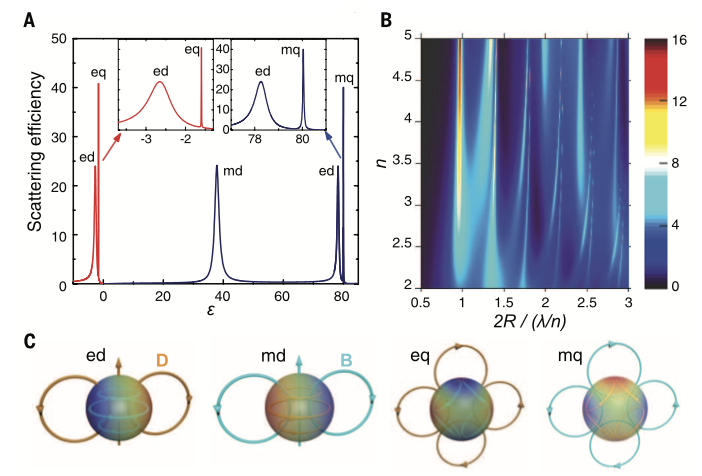
\includegraphics[width=0.7\linewidth]{images/fig1.png}
	\caption{\textbf{(a)}Эффективность рассеяния (безразмерное отношение сечения рассеяния к геометрическому сечению частицы) в зависимости от диэлектрической проницаемости $\varepsilon$ (частицы без потерь, q = 0,5) для плазмонных ($\varepsilon$  < 0) и диэлектрических ( $\varepsilon$ > 0) материалов. Сокращения для резонансов: ed - электрический диполь; eq - электрический квадруполь; md - магнитный диполь; mq - магнитный квадруполь. \textbf{(b)} Эффективность рассеяния диэлектрической частицы без потерь (цветная шкала справа) как функция показателя преломления n и параметра размера. \textbf{(c)} Иллюстрация структур электрического и магнитного поля для различных электрических и магнитных резонансов, поддерживаемых сферической диэлектрической частицей. Графики взяты с \cite{kuznetsov2016optically}}
	\label{fig1}
\end{figure}
\hspace*{2mm}
Чтобы проиллюстрировать фундаментальные свойства рассеяния света наночастицами, рассмотрим случай сферической частицы, освещенной плоской волной, для которой существует точное аналитическое решение уравнений Максвелла. Согласно теории Ми \cite{absorbScattLight}, металлические и диэлектрические сферические частицы могут обладать сильными резонансами рассеяния (рис. \ref{fig1}a). В случае немагнитных материалов их свойства рассеяния зависят только от двух параметров: диэлектрической проницаемости $\varepsilon$  и размерного параметра q ($q = 2\pi R/\lambda$). Различие между металлическими и диэлектрическими частицами заключается в знаке диэлектрической проницаемости, которая является отрицательной для металлов и положительной для диэлектриков. Небольшие металлические сферы (q < 1) создают только локализованные поверхностные плазмонные резонансы электрического типа:  дипольные, квадрупольные и т.д., в то время как их магнитный отклик остается практически незначительным из-за малого поля внутри сферы (рис. \ref{fig1}a).  
\\
\hspace*{2mm}
Чтобы воспроизвести "ощутимый" магнитный отклик от металлических структур, геометрия частицы должна быть другой. Например, резонатор с вырезанным кольцом \cite{pendry1999magnetism} работает аналогично LC-схеме (цепи индуктор-конденсатор), в которой усиление магнитного поля происходит в центре него. Для диэлектрических наночастиц наблюдается как электрический, так и магнитный отклики (рис. \ref{fig1}a). Резонансный магнитно-дипольный отклик является результатом взаимодейсвия входящего света с круговыми токами смещения электрического поля частицы. Это происходит, когда длина волны внутри частицы становится сопоставимой с диаметром частицы $2R \approx \lambda/n$ (рис. \ref{fig1}b) \cite{kuznetsov2016optically}. 
\\
\hspace*{2mm}
Полевая структура четырех основных резонансных мод диэлектрических частицах с высоким индексом приломления показана на рисунке \ref{fig1}c. На длине волны магнитного резонанса возбужденная магнитно-дипольная мода диэлектрической сферы с высоким показателем может вносить основной вклад в эффективность рассеяния, превосходя моды других мультиполей на порядки величины.
\\
\hspace*{2mm}
Из теории Ми следует, что максимально достижимая эффективность рассеяния для конкретного многополярного возбуждения субволновой частицы зависит только от резонансной частоты, а не от типа материала \cite{schuller2009general}. Это говорит о том, что многие плазмонные эффекты, наблюдаемые при рассеянии света металлическими наночастицами, могут быть реализованы с помощью диэлектрических наночастиц с высоким индексом преломления. На рисунке \ref{fig1}b показано масштабирование различных резонансов по отношению к показателю преломления n. При n > 2 все основные мультиполи хорошо определены, и их спектральные положения соответствуют фиксированному отношению длины волны внутри частицы к ее диаметру. Эффективность рассеяния всех мультиполей также увеличивается с ростом n \cite{articleOptSi}.

\subsection*{Наблюдение оптических магнитных резонансов в диэлектрических наночастицах.}
\hspace*{2mm}
Сильные оптически индуцированные магнитные дипольные резонансы в диэлектрических наночастицах с высоким индексом преломления могут быть достигнуты не только для сфер, но и для сфероидов \cite{articleDirVi}, \cite{optScatShper}, дисков и цилиндров \cite{multLightScat}, колец \cite{contrMagnModes} и многих других геометрий \cite{nearInfrMR}. Это обеспечивает важные возможности для создания разнообразных полностью диэлектрических наноструктур с желаемыми спектральными положениями резонансов. Спектральные положения как электрического, так и магнитного дипольного резонансов могут настраиваться независимо путем изменения формы частиц и расстояния между ними \cite{optScatDeilectrHightIndex}.
\\
\hspace*{2mm}
Кремниевые (Si) наносферы с размерами от 100 до 300 нм поддерживают сильные магнитные и электрические дипольные резонансы в видимой и ближней ИК областях спектра (рис. \ref{fig2}c). 
 \begin{figure}[h]
	\centering
	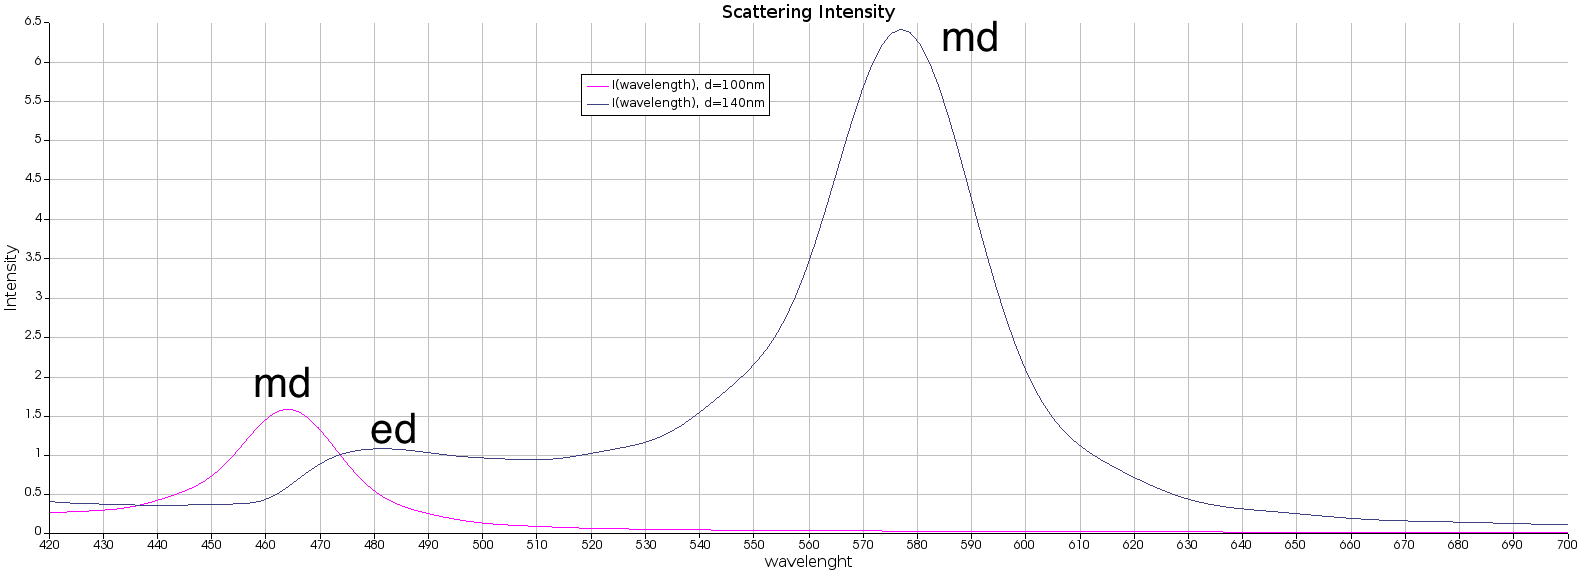
\includegraphics[width=1\linewidth]{images/graph1.png}
	\caption{\textbf{(a, b)} Изображения в темнопольном оптическом микроскопе (слева), изображения на сканирующем электронном микроскопе (SEM) (справа)  сферических наночастиц Si с приблизительными диаметрами 100 нм \textbf{(a)} 140 нм \textbf{(b)} \cite{kuznetsov2012luk}. \textbf{(c)} Результат моделирования оптического магнитного отклика наночастиц кремния  диаметром 100 нм. (синий график) и 140 нм. (оранжевый график).  Сокращения для резонансов: ed - электрический диполь; md - магнитный диполь}
	\label{fig2}
\end{figure}
Экспериментальная демонстрация электрических и магнитных дипольных резонансов на видимых длинах волн впервые была представлена для сферических наночастиц Si, полученных с помощью фемтосекундной лазерной абляции на кремниевых и стеклянных подложках \cite{kuznetsov2012luk}. 
\\
\hspace*{2mm}
Различные цвета, наблюдаемые на темнопольных микроскопах (рис. \ref{fig2}a, b), соответствуют магнитным дипольным резонансам почти идеальных сферических наночастиц Si с размерами от 100 до 200 нм \cite{kuznetsov2012luk}.  Помимо кремния, полупроводники группы IV и группы III-V с показателями преломления выше 2 могут иметь аналогичные оптические свойства в зависимости от их поглощения и показателя преломления в конкретном диапазоне длин волн. Например, магнитные и электрические дипольные резонансы недавно были экспериментально обнаружены в нанодисках арсенида галлия (GaAs) в видимом спектре \cite{person2013demonstration}.


\section{Нелинейные оптические резонансны диэлектрических наноструктур}
\hspace*{2mm}
Усиление в ближнем поле электрического и магнитного отклика в полностью диэлектрических наноструктурах может привести к новым нелинейным эффектам. В частности, генерация второй и третьей гармоник (ГВГ и ГТГ), самоиндукция света и комбинационное рассеяние. Известно, что плазмонные резонансы, которые усиливают локальные электрические поля, усиливают нелинейно-оптические эффекты в металлических наноструктурах. В отличие от плазмоники, при резонансе диэлектрических наночастиц с высоким индексом преломления генерируется большее количество различных мод, которые в последствии могут привести к резкому увлечению интенсивности.

\subsection*{Генерация третьей гармоники в наночастицах кремния, обусловленная магнитным откликом}
\hspace*{2mm}
Усиленная ГТГ от нанодисков Si, демонстрирующих как электрический, так и магнитный дипольный резонансы, наблюдалась экспериментально \cite{shcherbakov2014enhanced}. 
\begin{figure}[h!]
	\centering
	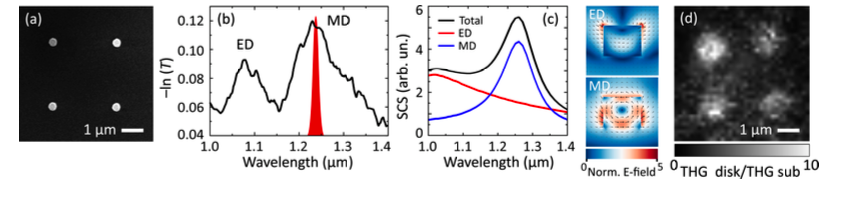
\includegraphics[width=1\linewidth]{images/fig4.png}
	\caption{Пространственно разделенные ГТГ от отдельных нанодисков Si, усиленных магнитным резонансом. \textbf{(а)} Изображение матрицы кремниевых нанодисков с d = 360 нм, h = 260 нм и p = 2,85 мкм. \textbf{(b)} Экспериментальный нормированный спектр пропускания образца (черный) со спектром импульса накачки, обозначенным красной областью. ED  обозначает положение электрического дипольного резонанса, а MD - положение магнитного дипольного резонанса. \textbf{(c) }Рассчитанные спектры сечения рассеяния нанодисков (черный), разложенных на электрические дипольные (красные) и магнитные дипольные (синие) вклады с соответствующими распределениями электрического поля. \textbf{(d)} Микроскопическое изображение образца. \cite{shcherbakov2014enhanced}}
	\label{nonliner:nanodisks1}
\end{figure}
\hspace*{2mm}
Диски освещались интенсивным фемтосекундным лазерным импульсом с частотой $\omega$, близкой к магнитно-дипольному резонансу первого. В результате высокой восприимчивости кремния третьего порядка $\chi^3$ передаваемый сигнал содержал импульсы утроенной основной частоты $3\omega$. Поскольку сигнал третьей гармоники (ТГ) пропорционален кубу локальной напряженности поля, разумно ожидать значительного усиления процесса ТГ в нанодисках с их магнитными резонансами, возбуждаемыми фундаментальной волной. (рис. \ref{nonliner:nanodisks}). 
\begin{figure}[h!]
    \centering
	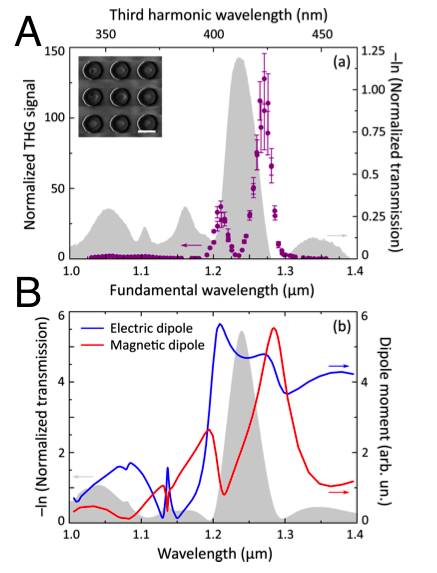
\includegraphics[width=0.8\linewidth]{images/fig3.png}
	\caption{\textbf{(a)}. ГТГ-спектроскопия массивов нанодисков Si. Отрицательный логарифм нормированного спектра пропускания образца с p = 0,8 мкм, h = 220 нм и d = 0,5 мкм показан серой областью, указывающей на резонанс при 1,24 мкм. Спектр ГТГ образца, нормированный по спектру подложки, показан фиолетовыми точками. На вставке показано изображение фрагмента образца. Масштабная линейка  500 нм. \textbf{(b)} Моделируемый спектр пропускания основной длины волны через диски и подложку, хорошо согласующийся с экспериментом. Наложенные синие и красные кривые дают величину электрических и магнитных дипольных моментов (соответственно). \cite{shcherbakov2014enhanced}}
	\label{nonliner:nanodisks}
\end{figure}
\hspace*{2mm}
Локализация поля в магнитном резонансе приводит к увеличению интенсивности гармоник на два порядка по отношению к неструктурированному объемному Si, при этом эффективность преобразования ограничивается только двухфотонным поглощением в подложке \cite{shcherbakov2014enhanced}. 


\section{Метаповерхности на основе резонансных металлических наноструктур.}
\hspace*{2mm}
Когда свет взаимодействует с металлическими наноструктурами, он  так-же  воздействуют с возбужденными свободными электронами вблизи поверхности металла. Электромагнитные резонансы, связанные с этими поверхностными плазмонами, зависят от геометрии наноструктуры. Результирующие резонансные электромагнитные поля позволяют значительно усилить слабые нелинейные процессы, которые суперлинейно зависят от локального поля.
\\
\hspace*{2mm}
Плазмонные возбуждения могут усиливать нелинейно-оптические эффекты несколькими способами. Во-первых, связь света с поверхностными плазмонами может приводить к усилению локальных электромагнитных полей \cite{novotny2011antennas}, которые значительно усиливают оптические процессы. Ярким примером является увеличение на несколько порядков процесса  комбинационного рассеяния. Во-вторых, плазмонные возбуждения могут быть чрезвычайно чувствительными к диэлектрическим свойствам. Это является основой для плазмонных датчиков: незначительные изменения показателя преломления вблизи поверхности металла приводят к значительным модификациям плазмонного резонанса \cite{homola2008surface}.
\\
\hspace*{2mm}
Нелинейные оптические эффекты возникают, когда электронное движение в сильном электромагнитном поле нельзя считать гармоническим. Наиболее важные эффекты возникают во втором и третьем порядке. 
\\
Отклик второго порядка обычно приводит к эффектам смешения волн, которые приводят к преобразованию частоты. Наиболее распространенным примером является генерация второй гармоники (ГВГ). Новые частоты возникают также из-за нелинейностей третьего порядка. Поверхностно-модулируемая вторая гармоника была впервые изучена с использованием поверхности серебра \cite{chen1981surface}. Сигнала второй гармоники был рассеянный, но довольно сильный. Результаты показали, что сигналы являются не когерентными и усиливаются резонансами наноразмерных поверхностных элементов. Дальнейшее подтверждение роли таких резонансов было получено из экспериментов генерации второй гармоники на пленках с металлическими вкраплениями \cite{wokaun1981surface}. Эти и дополнительные исследования показывают, что сигнал второй гармоники зависит от поляризации основного поля.
\\
Отклик третьего порядка содержит члены на падающих частотах - это называется оптическим эффектом Керра и приводит к нелинейным модификациям показателя преломления. Комбинируя нелинейности Керра с оптическими системами с обратной связью, можно получить бистабильность, когда один входной сигнал допускает два возможных выхода. Для оптических пучков с конечным поперечным размером дифракционные и нелинейные эффекты могут уравновешивать друг друга, создавая оптические солитоны.

\subsection*{Структурированные плазмонные поверхности для усиления нелинейных эффектов.}
\hspace*{2mm}
Первой плазмонной структурой, разработанной для генерации второй гармоники, была металлическая решетка, которая усиливала локальное поле на длине волны второй гармоники и вызывала эмиссию ГВГ  в первом дифракционном порядке \cite{grosse2012nonlinear}. 
\\
Первый пример нецентросимметричной поверхности состоял из массива L-образных наночастиц. Подобные массивы L-образных частиц золота были исследованы на способность генерации второй гармоники (рис. \ref{mettals}а). Было обнаружено, что эффективность сильно зависит от упорядочения частиц в решетке, причем самые сильные сигналы возникают, когда основная длина волны находится в плазмонном резонансе структуры. Резонаторы с расщепленным кольцом \cite{linden2012collective} (рис. \ref{mettals}b) имеют симметрию, аналогичную L-образным наночастицам. Плазмонные резонансы можно интерпретировать как имеющие электрический или магнитный характер, хотя сами составляющие материалы являются немагнитными. 
\\
\hspace*{2mm}
Генерация второй гармоники также обсуждалась для центросимметричных образцов, включая массивы наночастиц \cite{mcmahon2006second} и наноапертур. Во всех случаях наиболее сильная вторая гармоника была обнаружена, когда, по крайней мере, основной пучок или пучок ГВГ распространялся под косым углом падения. Вот, например, в недавней работе были продемонстрированы более совершенные плазмонные поверхности с улучшенными нелинейными свойствами. Кажущаяся центросимметрия диэлектрических решеток была нарушена для ГВГ из-за освещения металла под косым углом \cite{genevet2010large} (Рис. \ref{mettals}d). 
\\
\hspace*{2mm}
Наноструктурированные плазмонные поверхности также используются для усиления отклика известных нелинейных материалов. Один интересный образец состоял из массивов коаксиальных дырок в золотой пленке толщиной 70 нм на подложке из арсенида галлия (GaAs)  \cite{fan2006second}. Структуры демонстрировали отклик второй гармоники вблизи среза коаксиальной волноводной моды.

\begin{figure}[h!]
	\centering
	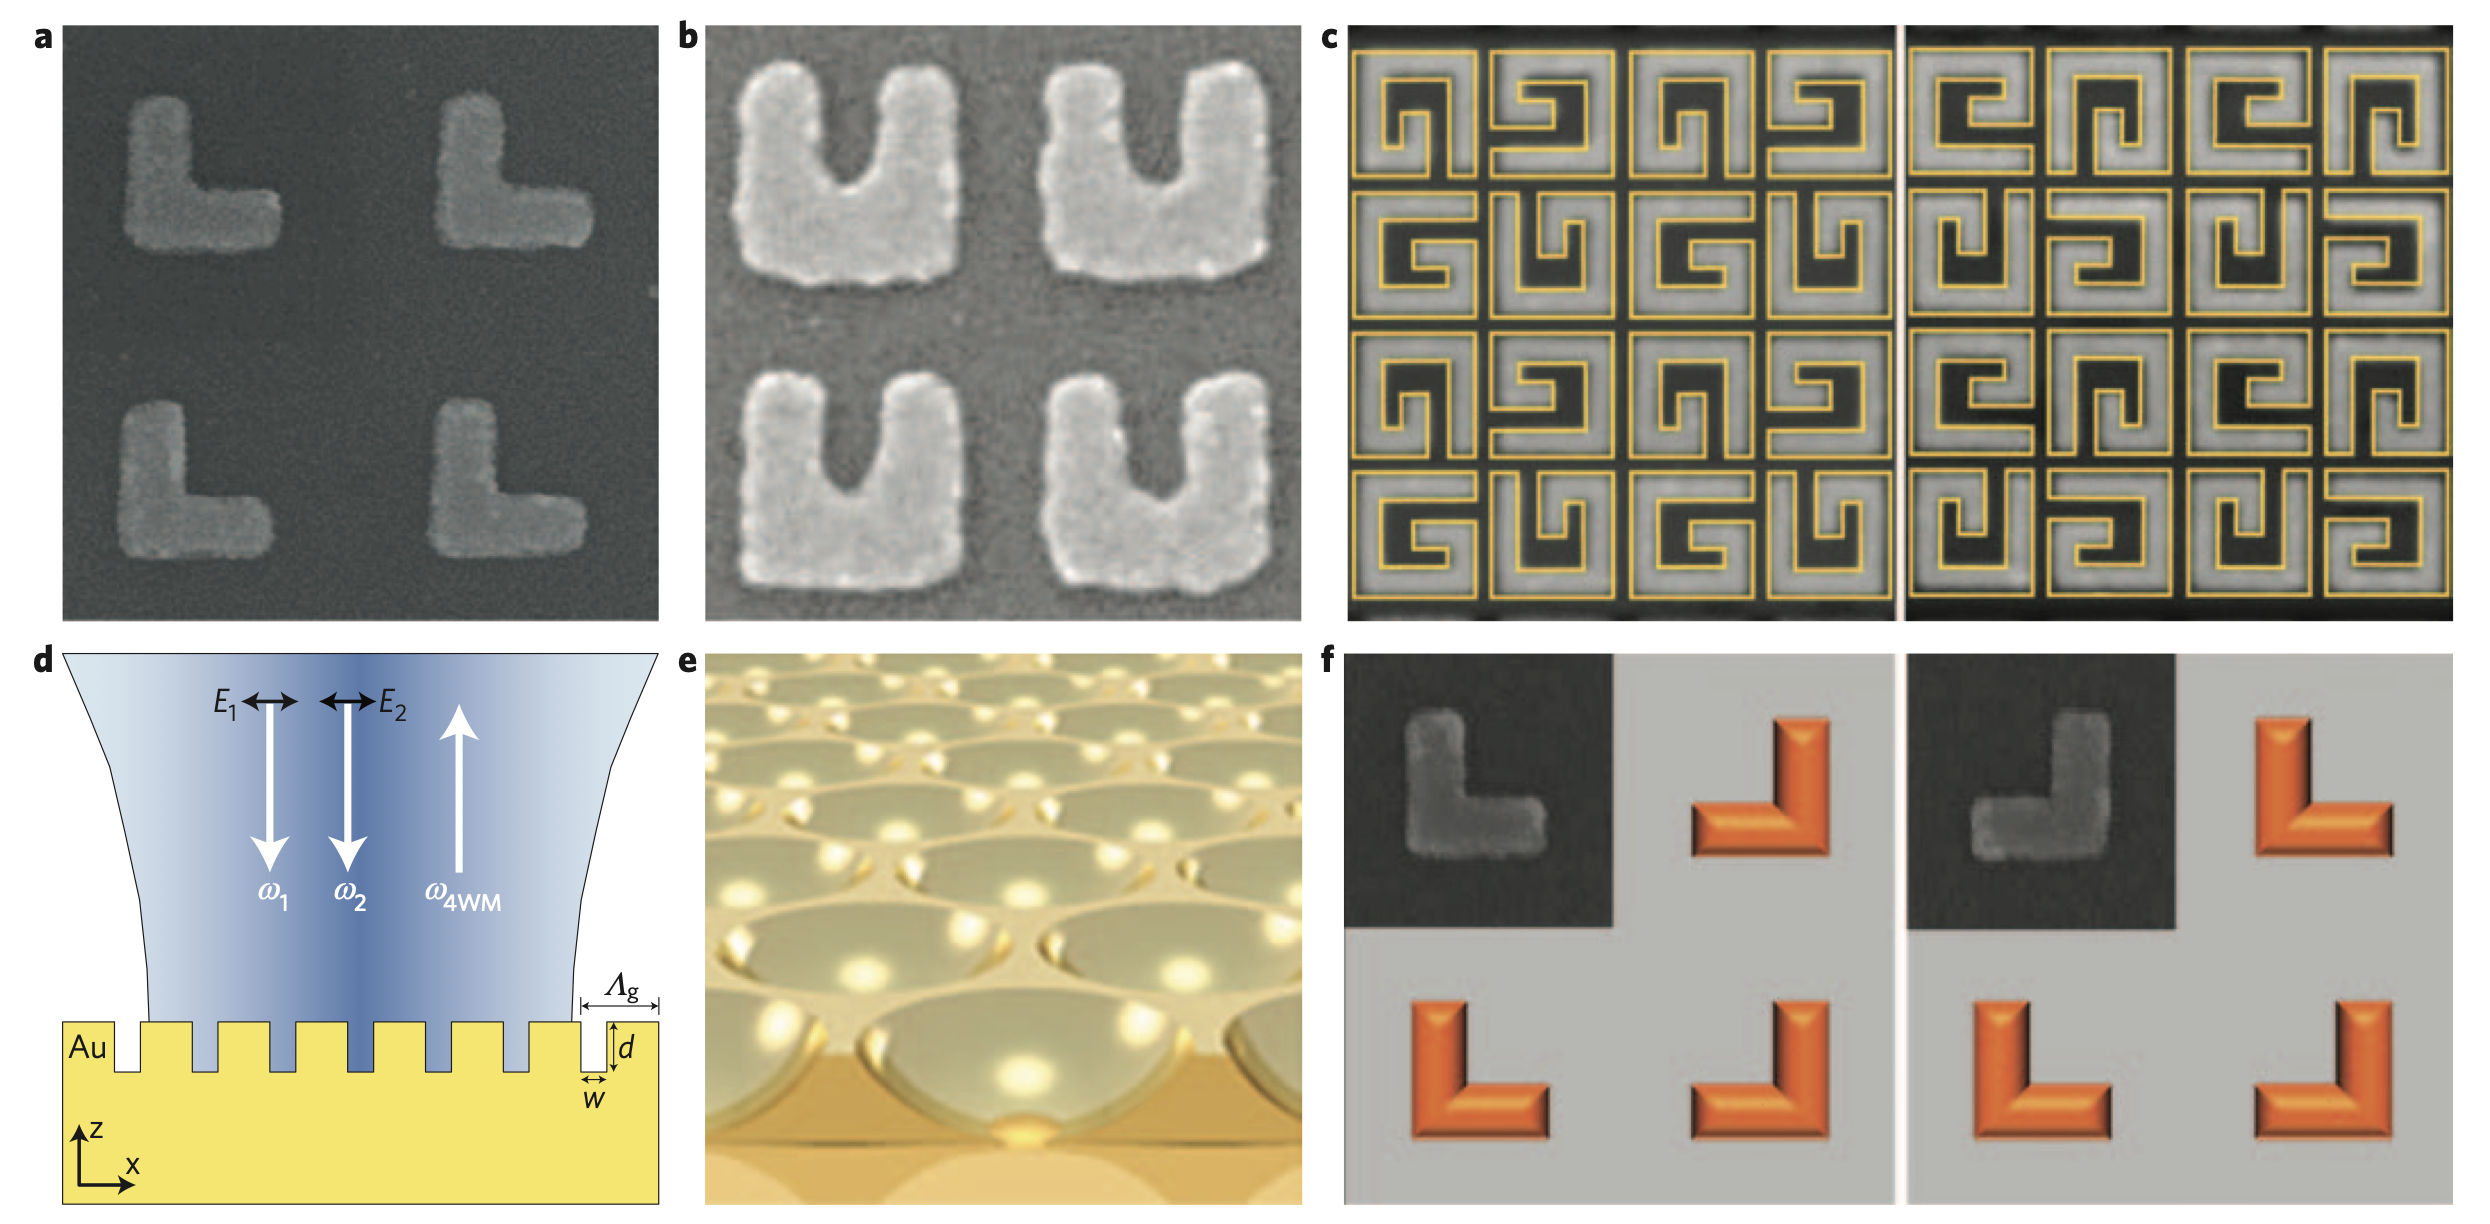
\includegraphics[width=0.9\linewidth]{images/mettals.png}
	\caption{Примеры структурированных металлических поверхностей для нелинейной плазмоники. \textbf{a – c}, Некоторые из основных случаев, исследованных для ГВГ: \textbf{(а)} L-образные частицы золота; \textbf{(b) }золотая структура; \textbf{(c)} По-разному упорядоченые G-образные хиральные частицы. \textbf{d – f},  Последние, более совершенные структуры для усиления нелинейных эффектов: золотая решетка для улучшения ЧСВ-сигала. Синяя часть представляет собою падающие поля E1 и E2 на соответствующих частотах $\omega_1$ и $\omega_2$, а также сгенерированный сигнал на частоте $4\omega_{WM}$. Желтая часть представляет собой золотую решетку с указанными критическими размерами; \textbf{(е) }нанополости золота для улучшенных CARS; (f) изменение порядка L-образных частиц может подавлять или усиливать ГВГ.}
	\label{mettals}
\end{figure}

\hspace*{2mm}
Точно так же массив сферических нанополостей в золотой пленке используют для спектроскопии(рис. \ref{mettals}e). Массивы частиц использовались для генерации высших гармоник вплоть до семнадцатой гармоники \cite{kim2008high} и для усиления некоторых других нелинейных процессов. Наконец, сигнал второй гармоники  был улучшен путем упорядочения частиц (рис. \ref{mettals}f), что привело к 50-кратной разнице в сигналах второй гармоники, которые, как ожидается, должны были быть эквиваленты.

\section{Метаповерхности на основе резонансных диэлектрических наноструктур.}
\hspace*{2mm}
Резонансные диэлектрические наночастицы также могут быть использованы для создания плоских однослойных решеток, известных как метаповерхности \cite{yu2014flat}. Использование метаповерхностей позволяет наблюдать различные резонансы  электрического и магнитно-оптического отклика в сочетании с низкими потерями тонкослойных структур. Одной из основных функций метаповерхностей является контроль фазы отраженного и прошедшего света. Идея использования диэлектриков, структурированных в масштабе длины волны для управления волновым фронтом, активно обсуждалась раньше \cite{lalanne1999design}. Надо сказать, что для достижения  2-фазного накопления подобные идеи также были реализованы и на сегодняшний день эти решения обеспечивает хорошую эффективность.
\\
\hspace*{2mm}
Другой подход к достижению фазового контроля был предложен в начале 2000-х годов, и он опирается на металлические или диэлектрические субволновые решетки. Недавняя работа, основанная на этом принципе, продемонстрировала плоские кремниевые линзы и аксиконы, работающие на видимых длинах волн (рис.  \ref{nonliner:matasurf1}a) \cite{lin2014dielectric}. 
\\
\hspace*{2mm}
Новым подходом к созданию диэлектрических метаповерхностей является использование электрических и магнитных дипольных резонансов диэлектрических наночастиц для контроля фазы входящего света \cite{shalaev2015high}. Каждый из диполей способен сдвигать фазу от 0 до $\pi$ вблизи резонанса. Объединение отклика обоих диполей на одной и той же длине волны позволяет достичь полного покрытия \cite{decker2015high}. Такое перекрытие резонансов обеспечивает не только необходимые фазовые сдвиги, но и подавление обратного рассеяния, из-за первого условия Керкера.
 \begin{figure}[h!]
	\centering
	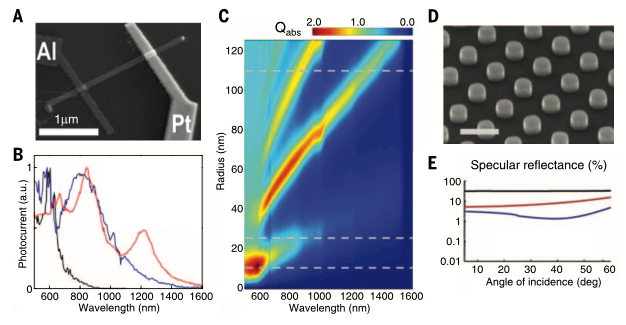
\includegraphics[width=0.8\linewidth]{images/fig5.png}
	\caption{ Нанофотонные устройства на основе полупроводниковых наноантенн. \textbf{(a)} Изображение фотодетектора с использованием оптически резонансной нанопроволоки Ge с асимметричными металлическими контактами. \textbf{(b)} Фототоковые спектры отдельных нанопроволок Ge с радиусами 10 нм (черный), 25 нм (синий) и 110 нм (красный). \textbf{(c)} Двумерный график рассчитанной эффективности поглощения как функции длины волны и радиуса нанопроволоки. Пунктирные серые линии указывают радиусы, для которых спектральный фототок показан в \textbf{(b). (d)} Изображение матрицы резонаторов Si, которая служит антибликовым покрытием на подложке Si \cite{spinelli2012broadband}. Масштабная линейка 1 мм. \textbf{(e)} Измерение зеркального отражения при 632 нм в зависимости от угла падения для непокрытой пластины Si (черного цвета), с антиотражающем покрытием Si3N4 толщиной 60 нм (красного цвета) и матрицы резонаторов Ми, как показано на \textbf{(d)} покрытый слоем $Si_3N_4$ толщиной 60 нм (синий) \cite{spinelli2012broadband}. }
	\label{nonliner:matasurf1}
\end{figure}
\\
\hspace*{2mm}
Такие конструкции концептуально аналогичны метаповерхностям Гюйгенса, предложенным в плазмонике \cite{pfeiffer2014efficient}, но они имеют гораздо более высокую эффективность пропускания из-за меньших потерь в прозрачных диэлектрических материалах. Недавно были продемонстрированы экспериментально мета-поверхности видимого диапазона на основе кремния с резонансным пропусканием более 85\%. Эти устройства имеют толщину всего 130 нм, что соответствует менее чем одной пятой длины волны в свободном пространстве, и способны контролировать волновой фронт света и выполнять отклонение луча с эффективностью передачи, близкой к 50\% (рис. \ref{nonliner:matasurf1}, b и c). Аналогичные концепции были также использованы для достижения эффективной генерации вихревого пучка (рис. \ref{nonliner:matasurf1}d). 
\\
\hspace*{2mm}
Диэлектрические поверхности также могут быть использованы в качестве практически идеальных отражателей \cite{moitra2015large},\cite{nearRefcLayer}.  Эффект отражения возникает в результате когерентного взаимодействия магнитных или электрических диполей, возбуждаемых внешним излучением в каждой наночастице. Недавний эксперимент продемонстрировал очень высокий коэффициент отражения (до 99,7\%) в ближней ИК-области спектра от плотного массива наночастиц Si \cite{moitra2015large}. Такое поведение с высоким коэффициентом отражения концептуально аналогично тому, которое наблюдалось ранее в высококонтрастных решетках с субволновой длиной. 
\\
\hspace*{2mm}
Другим примером является обобщенный эффект Брюстера. В отличие от обычного эффекта Брюстера, который ограничен p-поляризованным падением и углами выше $45^\circ$ (угол Брюстера ниже $45^\circ$ всегда сопровождается полным внутренним отражением под большими углами), обобщенный эффект Брюстера может быть достигнут для любой поляризации (как p, так и s) и любой угол падения (как ниже, так и выше $45^\circ$ без полного внутреннего отражения) (рис. \ref{nonliner:matasurf1}e). Оно возникает в результате интерференции электрических и магнитных резонансов в решетке и подавления их рассеяния в направлении отражения.

\subsection*{Возбуждение второй гармоники с использованием нарушенной симметрии III - V полупроводниковых метаповерхностей Фано}

\hspace*{2mm}
Схема Фано-резонансной мета-поверхности показана на рисунке  \ref{nonliner:matasurf}а. Форма нанорезонатора приводит к смешению мод между поперечными и продольными дипольными модами света, что приводит к резонансу Фано с высокими значениями добротности. Эти резонансы могут наблюдаться как в спектре  пропускания так и в спектре отражения.

\begin{figure}[h!]
    \centering
	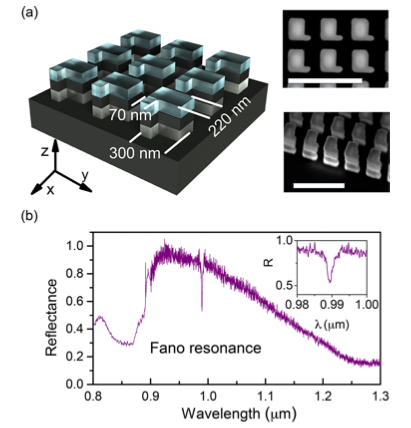
\includegraphics[width=0.5\linewidth]{images/fig6.png}
	\caption{Несимметричная мета-поверхность GaAs используется для создания резонансов Фано с высоким Q. \textbf{(а) }Схема фанорезонансной структуры мета-поверхности, основанная на кубе со стороной $\approx 300$ нм, который имеет угловой вырез. Верхняя часть вставки - изображение метаповерхности Фано. Вставка снизу: изображение метаповерхности, полученное под углом $20^\circ$. Масштабная линейка соответствует 1 мкм. \textbf{(b)} Спектр отражательной способности мета-поверхности Фано, который обладает высоким Q-резонансом с шириной спектра $\approx$ 2 нм. Вставка представляет собой увеличенную область спектра отражения вокруг резонанса Фано. \cite{vabishchevich2018enhanced}}
	\label{nonliner:matasurf}
\end{figure}

Резкий провал в спектрах отражения на рис. \ref{nonliner:matasurf}b при $\lambda_{F} \sim0,99$  мкм соответствует возбуждению резонанса Фано со спектральной шириной $\Delta\lambda_{F} \sim 2$ нм (добротность$\lambda_{F} /\Delta\lambda \sim 500$)). Численные расчеты показывают, что в идеальной наноструктуре усиление электрического поля внутри нанорезонатора при резонансе Фано достигает значения $|E|^2/|E_{0}|^2 \sim 500$. На рис. \ref{nonliner:matasurf2}а показана интенсивность сигнала второй гармоники, генерируемого  ассиметричной мета-поверхностью GaAs. Спектр интенсивности ГВГ имеет узкий пик при $\sim$ 0,99 мкм, который соответствует положению резонанса Фано в линейном спектре. Из-за локализации электромагнитного поля и увеличения его интенсивности, внутри нанорезонатора сигнал ГВГ  (когда лазер накачки настроен на резонанс Фано) в  $\sim$ 300 раз сильнее по сравнению с нерезонансным случаем. На рисунке \ref{nonliner:matasurf2}A показан сценарий модификации нормализованного спектра ГВГ, когда длина волны несущей накачки отрегулирована относительно резонансной длины волны. Когда $\Delta\lambda_{F} = -10$ нм, перекрытия с резонансом Фано не происходит, и форма генерируемой второй гармоники близка к гауссовой .На рис. \ref{nonliner:matasurf2}B показано сравнение спектра второй гармоники, полученного на мета-поверхности GaAs при накачке на длине волны Фано-резонанса, и ВГ, генерируемая в неповрежденной области подложки GaAs. 
 \begin{figure}[h!]
	\centering
	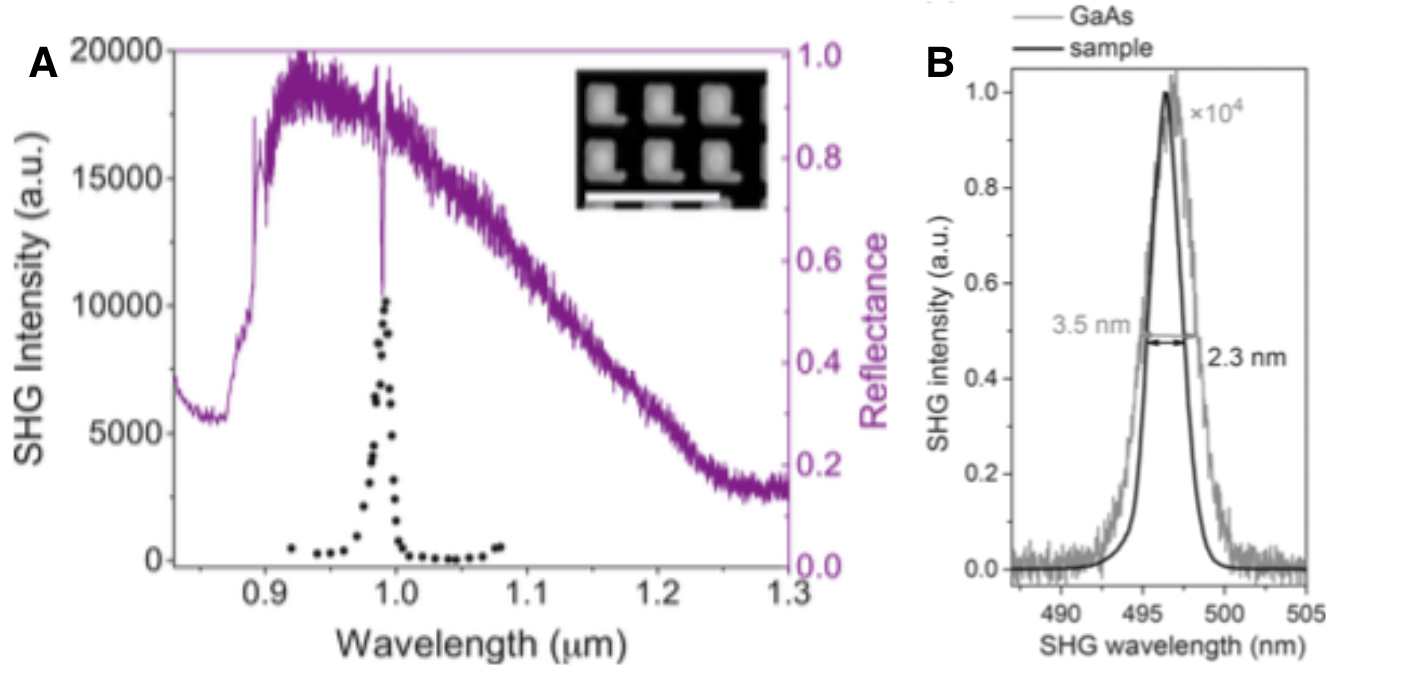
\includegraphics[width=0.7\linewidth]{images/fig7.png}
	\caption{\textbf{(a): }Генерация второй гармоники (ГВГ) на резонансной поверхности Фано. Точки: экспериментальная спектральная зависимость интенсивности ГВГ, демонстрирующая резонансно усиленную ГВГ на длинах волн резонанса Фано. Фиолетовый: линейный спектр отражения мета-поверхности Фано. Вставка: вид сверху образца SEM. \textbf{(b):} Сужение спектров SH, генерируемых мета-поверхностью Фано (черная линия), по сравнению с SH, генерируемым непокрытой подложкой GaAs (серая линия) \cite{vabishchevich2018enhanced}}
	\label{nonliner:matasurf2}
\end{figure}


\subsection*{Использование диэлектрических метаповерхностей как широкополосный оптический частотный смеситель}
\textit{Частотный смеситель} - это нелинейное устройство, которое объединяет электромагнитные волны для создания волн на новых частотах. Эти устройства широко используются в  современных радиочастотных технологиях и в обработке микроволновых сигналов. Разработка универсальных частотных смесителей для оптических частот остается сложной задачей: такие устройства обычно полагаются на слабые нелинейные оптические процессы и, таким образом, должны удовлетворять условиям согласования фаз.
\\
\hspace*{2mm}
Рассмотрим диэлектрическую метаповерхность на основе GaAs. Оптический смеситель на ее основе способен одновременно генерировать одиннадцать новых частот, охватывающих ультрафиолет и почти инфракрасный диапазоны. Нелинейности четного и нечетного порядка GaAs позволяют наблюдать генерацию \textit{второй гармоники}, \textit{третьей гармоники} и \textit{четвертой гармоники}, \textit{генерацию суммарной частоты}, \textit{двухфотонную фотолюминесценцию}, вызванную поглощением,\textit{ четырехволновое и шестиволновое смешение}. Одновременному возникновению этих семи нелинейных процессов помогают комбинированные эффекты сильных внутренних нелинейностей материала, усиленных электромагнитных полей и ослабленных требований к фазовому согласованию.
\\
\hspace*{2mm}
На рис. \ref{mixerPictr1}а приведена схема генерации нелинейной частоты метаповерхностью GaAs, накачиваемой двумя лазерными лучами. Метаповерхность состоит из периодической квадратной матрицы наноцилиндров диаметром $\sim 400$нм. Каждый наноцилиндр состоит из трех слоев: верхний надодиск из $SiO_x (\sim 300 $нм), средний нанодиск из GaAs толщиной $\sim 450$нм, в которым будет ограниченно электромагнитное поле, и нижний слой из $(Al_xGa_{1 - x})_20_3 \sim 400$нм с низким показателем преломления  для того чтобы отделить весь цилиндр от подложки.
\\
\hspace*{2mm}
Резонансное усиление частот достигается за счет одновременного  возбуждения магнитных дипольных (MD) и электрических дипольных (ED) Ми-резонансов наноцилиндра GaAs \cite{liu2016iii}. В измеренном спектре отражатения (рис. \ref{mixerPictr1})b наблюдались максимумы при $\lambda_{ED} \sim 1,25$мкм и $\lambda_{MD} \sim 1,5$мкм, которые соответствуют возбуждению резонансов ED и MD. Это  подтверждается выполнением многополярным разложением полей рассеяния, а также моделированием профилей электрического поля (показано на вставках) для двух длин волн, которые соответствуют максимальному усилению электромагнитного поля внутри нанорезонаторов (1,246 мкм и 1,535 мкм).
\begin{figure}[h!]
	\centering
	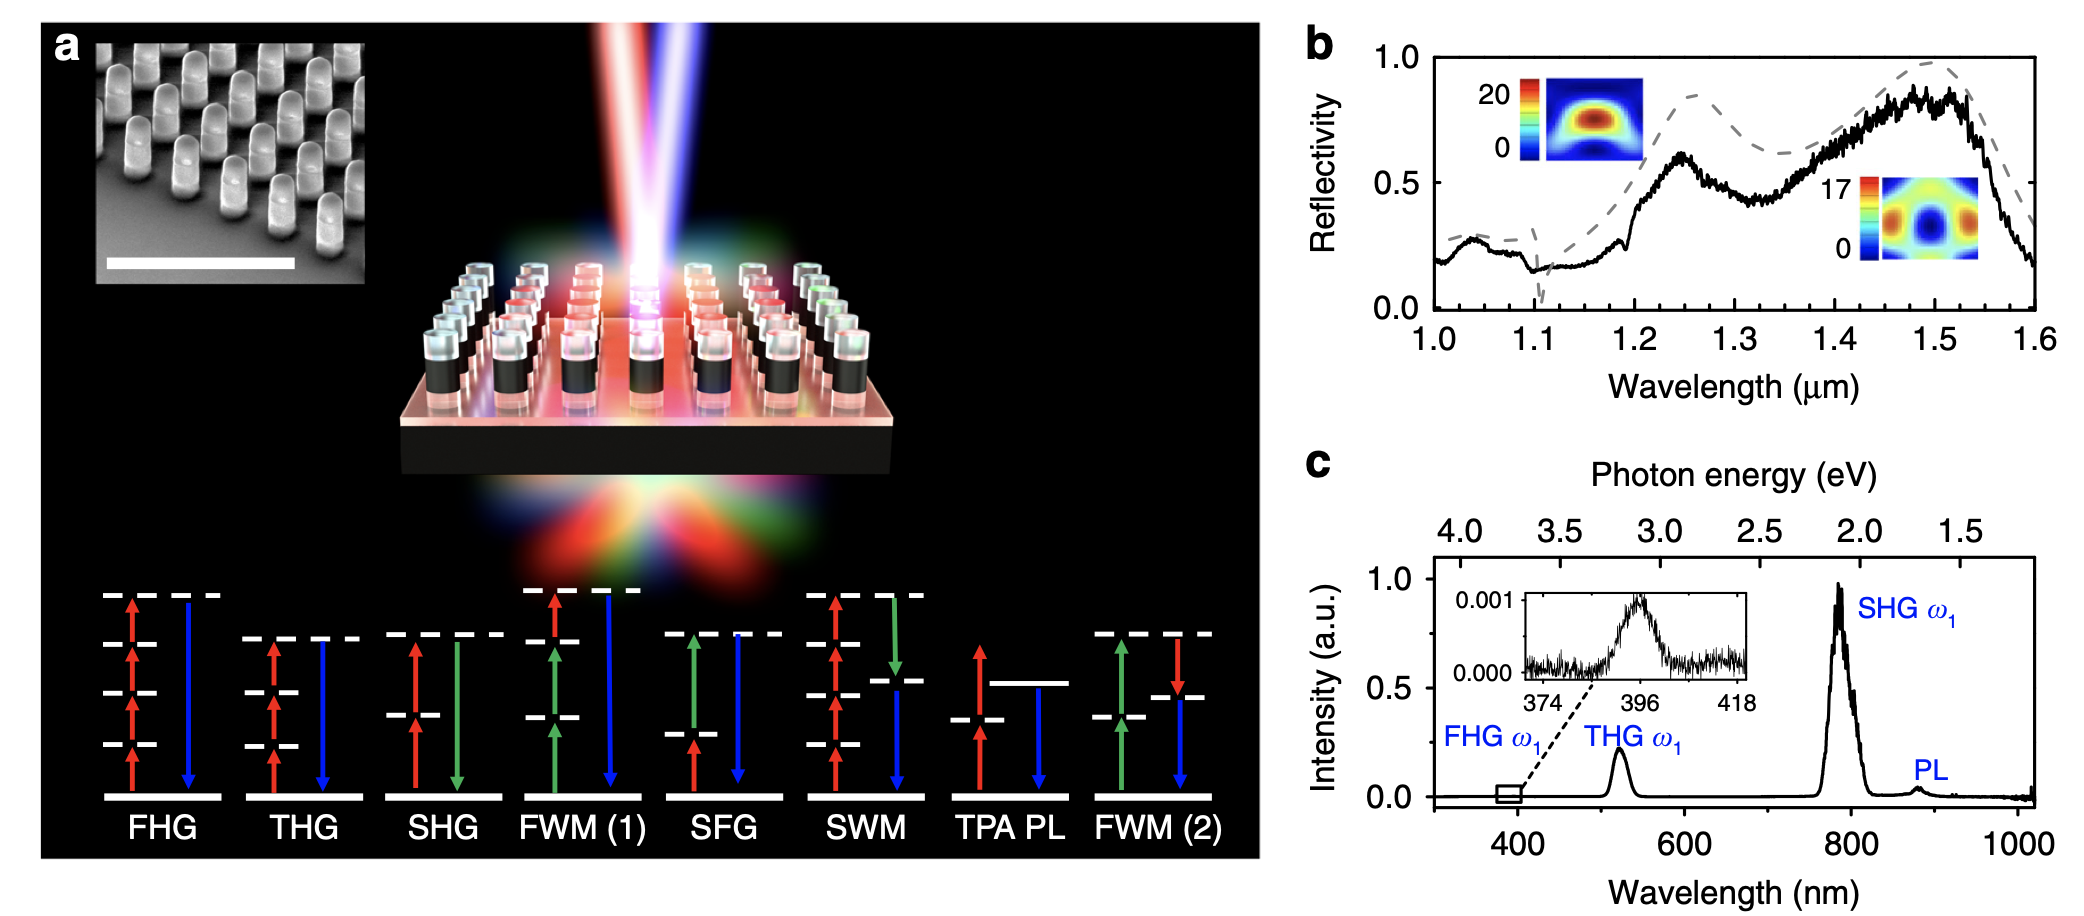
\includegraphics[width=0.7\linewidth]{images/mixer.png}
	\caption{Генерация новых частот с помощью метаповерхностью из  GaAs. Схема оптического метамиксера, состоящего из квадратной матрицы субволновых диэлектрических резонаторов. \textbf{(a):} Два фемтосекундных ближних ИК-импульса накачивают метамиксер, и одновременно генерируется множество новых частот. Вставка: изображение сканирующего электронного микроскопа под углом 60 $^\circ$ поверхности GaAs. Масштабная линейка соответствует 3 мкм. Нижняя вставка: схематические энергетические диаграммы семи нелинейных оптических процессов, которые происходят одновременно в эксперементе: генерация второй гармоники (ГВГ), генерация третьей гармоники (ГТГ), генерация четвертой гармоники (ГЧГ), генерация суммарной частоты (ГСЧ) фотолюминесценция, индуцированная двухфотонным поглощением (TPA PL), четырехволновое смешение (ЧВС) и шестиволновое смешение (ШВС). \textbf{b} Измеренные (сплошная линия) и численно смоделированные (пунктирная линия) спектры отражения метаповерхности с двумя поперечными локальными распределениями электрического поля на длинах волн 1,246 мкм и 1,535 мкм, которые соответствуют максимальным усилениям электромагнитного поля внутри нанодиска GaAs. \textbf{(c)} Спектры второй, третьей и четвертой гармоник, когда импульсы накачки $\lambda_1 \sim $1,57 мкм используются для возбуждения метамиксера. Вырезка - это увеличение четвертой гармоники \cite{liu2018all}}
	\label{mixerPictr1}
\end{figure}
\\
\hspace*{2mm}
\textbf{Генерация гармоник в однолучевых экспериментах}. При накачке одним фемтосекундным лучом с длиной волны в близи MD резонанс ($\lambda_1 \sim$ 1,57 мкм)  генерируются вторая($\lambda_{SHG} \sim$ 785 нм), третья($\lambda_{THG} \sim$ 523 нм) и четвертая($\lambda_{FGH} \sim$ 393 нм) гармоники (рис. \ref{mixerPictr1}с) . Излучение с центром при $\lambda_{PL} \sim$ 870 нм соответствует GaAs-фотолюминесценции (PL), возникающей при двухфотонном поглощении (TPA) накачки. Наблюдаемые гармоники лежат выше энергии запрещенной зоны GaAs и поэтому значительная часть их излучения поглощается.
\\
\hspace*{2mm}
\textbf{Смешивание частот в двухлучевых экспериментах}.  Когда два пучка накачки (первый - $\lambda_1 \sim$ 1,57 мкм, второй - $\lambda_2 \sim$ 1,24)  совпадают во времени, мы наблюдаем одиннадцать спектральных пиков в диапазоне от $\sim$ 380 до  $\sim$ 1000 нм (рис. \ref{mixerPictr2}а).  Сгенерированные сигналы можно условно разделить на две группы:
\\
Первая группа (обозначенная синими метками) соответствует процессам генерации гармоник, а также PL, возникающим при двухфотонном поглощении. Каждый из процессов в этой группе опирается только на один пучок накачки. 
\\
Напротив, вторая группа (обозначенная красными метками) соответствует процессам смешивания частот, которые требуют обоих импульсов накачки. Пять сигналов смешивания частот включают в себя: генерацию суммарной частоты $(\omega_1 + \omega_2)$ при $\lambda_{SHG} \sim$ 689 нм; три типа четырехволнового смешения $(2\omega_1 + \omega_2, 2\omega_2 + \omega_1, 2\omega_2 - \omega_1)$при $\sim$ 1000 нм, $\sim$ 472 нм и $\sim$ 434 нм соответственно; и шестиволновое смешение $(4\omega_1 - \omega_2)$ при $\lambda_{SWM} \sim$ 577 нм. Отметим, что амплитуда пика ЧВС $(2\omega_2 - \omega_1)$ как минимум в десять раз выше, чем у любого другого нелинейного процесса. Это объясняется гораздо меньшим поглощением ниже запрещенной зоны у  GaAs в отличие от сильного затухания, испытываемого другими сигналами. В целом спектры содержат одновременные вклады, возникающие в результате семи нелинейно-оптических процессов .
\\
Проверим  физическое происхождение процессов новых частот путем измерения выходных спектров для различных длин волн накачки и для разных мощностей накачки. Например, выход ГСЧ идентифицируется по его энергии, совпадающей с суммой энергий фотонов двух пучков накачки $\omega_{SWG} = \omega_1 - \omega_2$, а также по линейной зависимости интенсивности от мощности одного накачки при мощности другого накачки поддерживается постоянным (рис. \ref{mixerPictr2}b, черная кривая). Аналогичным образом выполним измерения зависимости мощности для проверки процессов четырех- и шести-волнового смешения.

\begin{figure}[h!]
	\centering
	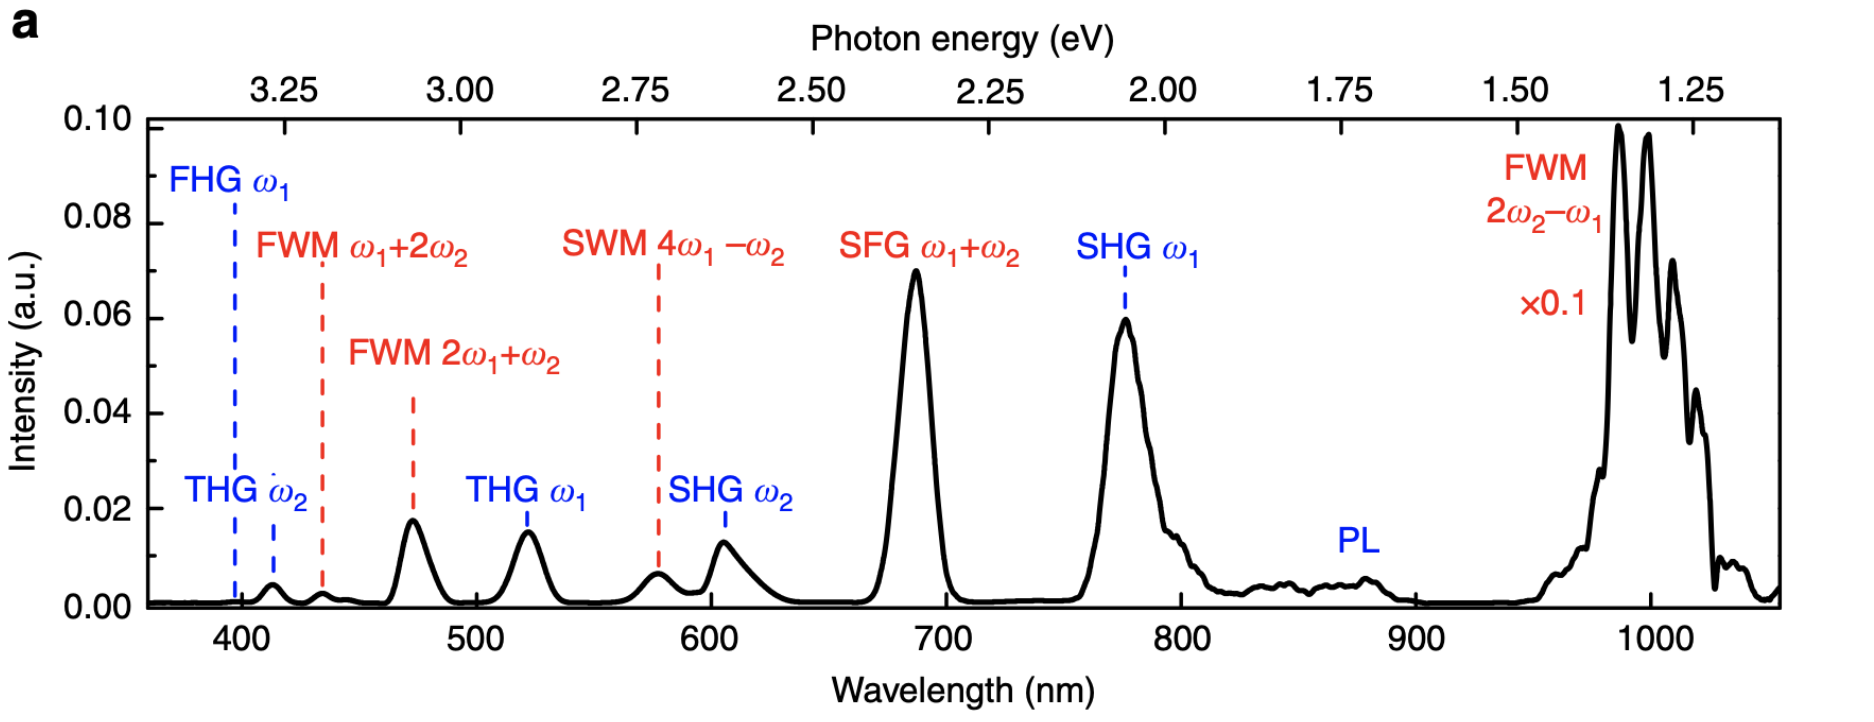
\includegraphics[width=0.8\linewidth]{images/mixer1.png}
	\caption{\textbf{(a)} Смешивание частот в метаповерхности GaAs. Спектр, демонстрирующий одиннадцать нелинейно генерируемых пиков, возникающих в результате семи различных нелинейных процессов, когда два оптических луча с  $\lambda_2 \sim$ 1,24 мкм и  $\lambda_1 \sim$ 1,57 мкм используются для одновременной накачки метаповерхности GaAs. Синие метки указывают на процессы генерации гармоник и фотолюминесценции, возникающие в результате двухфотонного поглощения, для каждого из которых требуется только один луч накачки. Красные метки указывают на частоты, которое включает оба луча насоса. \textbf{b}, Зависимость генерации суммарной частоты $(\omega_1 + \omega_2)$, четырехволнового смешения ($2\omega_2 - \omega_1)$ и шестиволнового смешения $(4\omega_1 - \omega_2)$ от мощности накачки $\omega_2$.\textbf{(c) } Показаны экспериментальные  точки и теоретическое предсказание (черная линия для линейной подгонки и красная кривая для квадратичной подгонки). \textbf{d} Пять спектров, показывающих настройку нормированного шестиволнового смешивающего сигнала $(4\omega_1 - \omega_2)$, когда длины волн накачки спектрально настроены на $\lambda_2 \sim$ 1248,7 нм,  $\lambda_1 \sim$ 1557,5 нм (черная кривая); $\lambda_2 \sim$ 1234,8 нм, $\lambda_1 \sim$1558,6 нм (красная кривая); $\lambda_2 \sim$1211,6 нм, $\lambda_1 \sim$ 1558,9 нм (синяя кривая); $\lambda_2 \sim$ 1234,9 нм, $\lambda_1 \sim$ 1581,2 нм (зеленая кривая); и $\lambda_2 \sim$ 1233,7 нм, $\lambda_1 \sim$1600,4 нм (пурпурная кривая). Стрелками обозначены теоретически ожидаемые частоты для рассматриваемого шестиволнового процесса смешения. \cite{liu2018all}}
	\label{mixerPictr2}
\end{figure}
\hspace*{2mm}
Экспериментальная демонстрация семи разных нелинейныхоптические процессы, происходящие одновременно в GaAs метаповерхности может быть использована для реализации ультракомпактных оптических смесителей. Видно, что нечетные нелинейные процессы высокого порядка могут генерировать гармоники высокого порядка, являющиеся основой генерации аттосекундных импульсов. Кроме того, эти метаповерхности могут быть оптимизированы для других нелинейных процессов смешивания, таких как генерация разностной частоты $\omega_{DFG} = \omega_1 - \omega_2$. Это позволило бы создавать фемтосекундные импульсы, охватывающие среднюю инфракрасную область спектра. 